
\documentclass{include/thesisclass3}

\SelectLanguage{ngerman}
\usepackage{float}
      

% Titlepage settings
\newcommand{\praktikum}{Praktikum moderne Physik}
\newcommand{\autora}{Jens Schäfer}
\newcommand{\autorb}{Jan van der Linden}
\newcommand{\maila}{ugecd@student.kit.edu}
\newcommand{\mailb}{jan.vdlinden95@gmail.com}
\newcommand{\topic}{Quantenradierer}
\newcommand{\ptime}{22. Mai 2017}


% Shortcuts
\newcommand{\cc}{\cdot}
\newcommand{\rk}{\rangle}
\newcommand{\lk}{\langle}
\newcommand{\df}{\rightarrow}
\newcommand{\la}{\lambda}
\newcommand{\dd}{{\rm d}}
\newcommand{\ehm}{\mathbbm{1}}
\newcommand{\p}{\partial}
\newcommand{\soll}{\overset{!}{=}}
\newcommand{\D}{\Delta}
\newcommand{\eps}{\epsilon}
\newcommand{\vektor}[3]{\begin{pmatrix} #1 \\ #2 \\ #3 \end{pmatrix}}
\newcommand{\vektorz}[2]{\begin{pmatrix} #1 \\ #2 \end{pmatrix}}
\newcommand{\Mat}[9]{\begin{pmatrix}#1&#2&#3\\#4&#5&#6\\#7&#8&#9\end{pmatrix}}
\newcommand{\Matz}[4]{\begin{pmatrix}#1&#2\\#3&#4\end{pmatrix}}
\newcommand{\e}[1]{\,\si{#1}}
 


\begin{document}

	\FrontMatter
	% coordinates for background border
\newcommand{\diameter}{20}
\newcommand{\xone}{-15}
\newcommand{\xtwo}{160}
\newcommand{\yone}{15}
\newcommand{\ytwo}{-253}




\begin{titlepage}
    % background border
    \begin{tikzpicture}[overlay]
    \draw[color=gray]
            (\xone mm, \yone mm)
      -- (\xtwo mm, \yone mm)
    arc (90:0:\diameter pt)
      -- (\xtwo mm + \diameter pt , \ytwo mm)
        -- (\xone mm + \diameter pt , \ytwo mm)
    arc (270:180:\diameter pt)
        -- (\xone mm, \yone mm);
    \end{tikzpicture}



    % KIT image and sign for faculty of physics
    \begin{textblock}{10}[0,0](4.5,2.5)
        
\includegraphics[width=.25\textwidth]{include/kitlogo.pdf}
    \end{textblock}
    

    % horizontal line
    \begin{textblock}{10}[0,0](4.2,3.1)
        \begin{tikzpicture}[overlay]
        \draw[color=gray]
                (\xone mm + 5 mm, -12 mm)
          -- (\xtwo mm + \diameter pt - 5 mm, -12 mm);
        \end{tikzpicture}
    \end{textblock}



    % begin of text part
    \changefont{phv}{m}{n}    % helvetica
    \centering



    % thesis topic (en and ge)
    \vspace*{3cm}
    \Huge\praktikum\\



    % author name and institute
    \vspace*{5cm}
    
    \huge\topic\\






    % examiners (Referenten)
    \vspace*{3cm}
    \Large
    \begin{center}
        \begin{tabular}[ht]{l c l } 
  \autora & \hfill & \textit{\maila} \\
\autorb & \hfill & \textit{\mailb} \\
        
        \end{tabular}
    \end{center}



    % working time
    \vspace{2cm}
    \begin{center}
        \large{Durchgeführt am}: \ptime
    \end{center}



    % lowest text blocks concerning the KIT
    \begin{textblock}{10}[0,0](4,16.8)
        \tiny{KIT -- Universität des Landes Baden-Württemberg und nationales %
              Forschungszentrum in der Helmholtz-Gemeinschaft}
    \end{textblock}
    \begin{textblock}{10}[0,0](14,16.75)
        \large{\textbf{www.kit.edu}}
    \end{textblock}
\end{titlepage}

	\tableofcontents                  
	\newpage
	\MainMatter

%Protokollstart

\chapter{Theoretische Grundlagen}

\section{Ziel des Experiments}

In diesem Experiment werden quantenmechanische Eigenschaften wie die Aufenthaltswarscheinlichkeit von Teilchen anschaulich dargestellt. Hierzu werden kohärente Photonen zur Interferenz im Mach-Zehnder-Interferometer gebracht. Der Quantenradierer ermöglicht hierbei die entstehung eines Interferenzpattern wobei dies mit der herkömmlichen Wellenmechanik nicht erklärbar wäre.

\section{Durchführung}
\begin{figure}[H]
	\begin{center}
		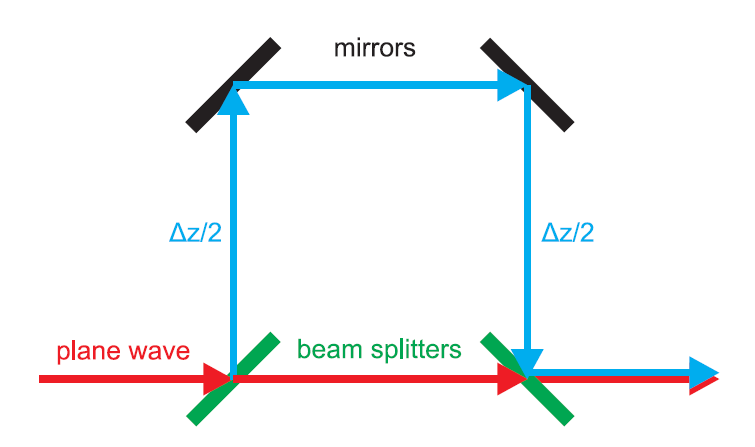
\includegraphics[width=0.8\textwidth]{images/Beamsplit.png}
		\caption{Mach-Zender-Interferometer, Quelle: Quantum Eraser, KSOP Optics \& Photonics Lab}
		\label{Mach-Zehnder}
	\end{center}
\end{figure}

In Abbildung \ref{Mach-Zehnder} ist ein Mach-Zehnder-Interferometer dargestellt. Ein Lichtstrahl wird dabei durch einen ersten Beamsplitter aufgeteilt. Der erste Strahl verläuft geradlinig weiter, der Zweite wird durch zwei Spiegel auf einen um $\Delta z/2$ längeren Umweg geführt. Nach dem Umweg werden die Teilstrahlen durch einen zweiten Beamsplitter wieder zusammengeführt, sodass sie fortan in einer Bahn weiter laufen. Als Lichtquelle wird ein Laser verwendet, somit sind die Teilstrahlen kohärent und gut fokusiert. Nach dem zweiten Beamsplitter bilden sich zwei Richtungen für die rekombinierten Strahlen aus, beide werden auf seperaten Schirmen abgebildet, wie in Abb. \ref{Aufbau} ersichtlich. 
\begin{figure}[H]
	\begin{center}
		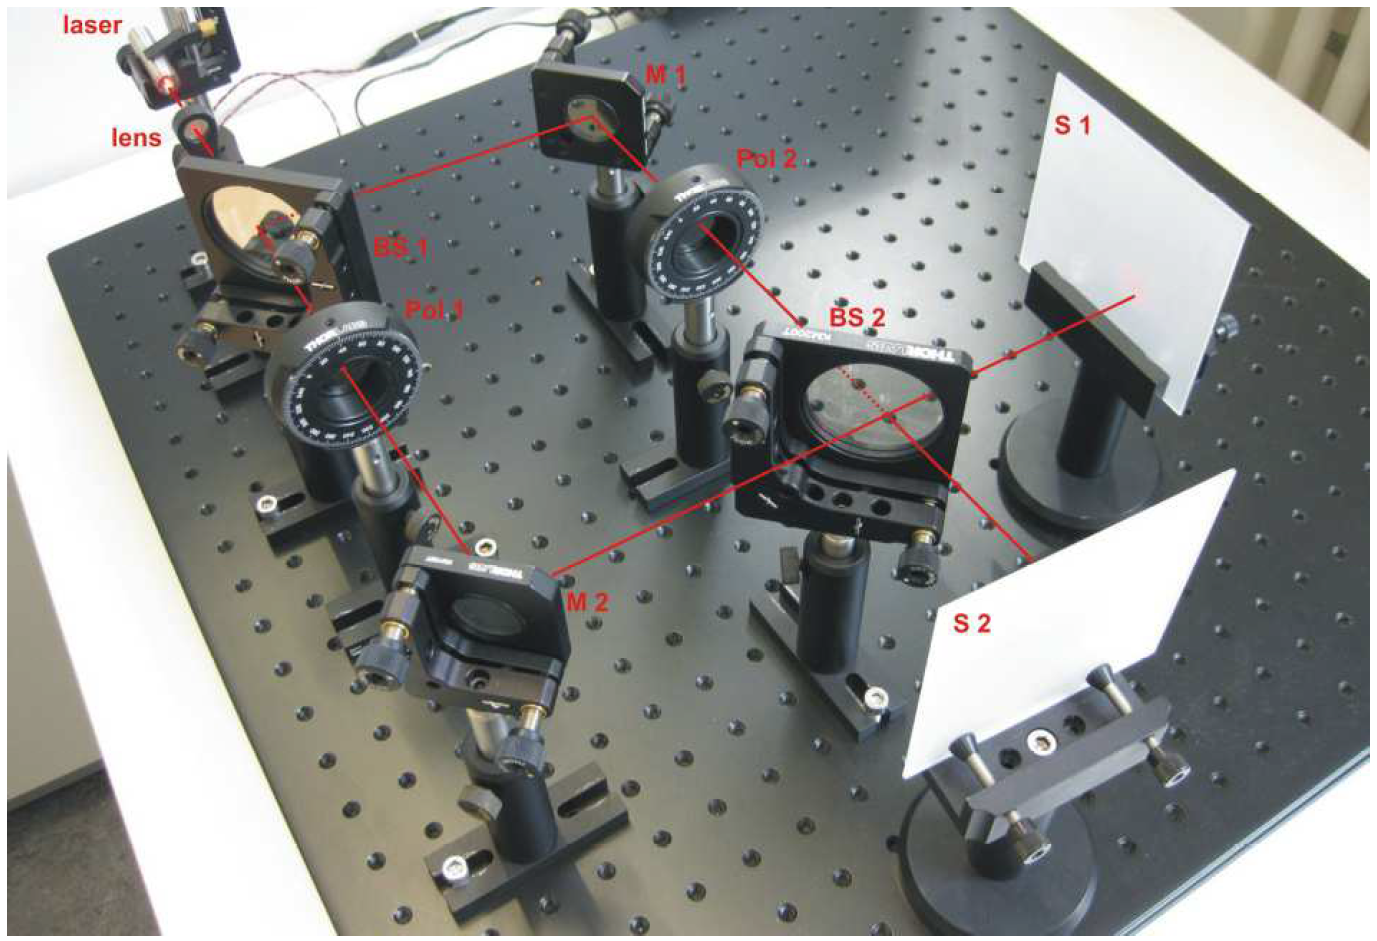
\includegraphics[width=0.8\textwidth]{images/Aufbau.png}
		\caption{Experimenteller Aufbau, Quelle: Quantum Eraser, KSOP Optics \& Photonics Lab}
		\label{Aufbau}
	\end{center}
\end{figure}
\subsection{Wellendynamik}
Die Photonendichte ist proportional zur Lichtintensität und gegeben mit:
\begin{equation}
n_{ph}(z,t)=\frac{I(\vec{x},t)}{\hbar \omega}=\frac{\vert \vec{E}\vert ^2}{\hbar \omega}
\end{equation}
Geht man von idealen Bedingungen aus, sollte klassisch gesehen die Teilchendichte sich nach aufteilen und wieder zusammenführen eines Strahls nicht verändern. Sei $\vec{E}_0$ die Feldstärke der Quelle. Bei dem Interferometer haben wir einen Gangunterschied zwischen den Teilstrahlen, welcher hinter dem zweiten Beamsplit wie folgt erfasst werden kann:
\begin{align}
\si{Strahl\, A}\quad \vec{E}_A(z,t)&=\frac{1}{4}\vec{E_0}e^{i(k_z z-\omega t)}\\
\si{Strahl\, B}\quad \vec{E}_B(z,t)&=\frac{1}{4}\vec{E_0}e^{i(k_z (z+\Delta z)-\omega t)}
\end{align}
Hierbei ist die Feldstärke eines jeden Teilstrahls auf ein Viertel abgesunken, da sie bei zwei Beamsplittern jeweils halbiert wurde. Nach zusammenführen der Teilstrahlen bekommt man die überlagerte Welle als Superpossition:
\begin{equation}
\vec{E}_{ges}(z,t)= \vec{E}_A+\vec{E}_B=\frac{1}{4}\vec{E_0}(e^{ik_z z}+e^{ik_z (z+\Delta z)})e^{i\omega t}
\end{equation}
Daraus ergibt sich die Photonendichte für einen der beiden rekombiniertenbeiden Strahlen hinter dem zweiten Beamsplitter zu:
\begin{equation}
n_{ph}(z,t)=\frac{\vert \vec{E}_{ges} \vert ^2}{\hbar \omega}=\frac{\vert \vec{E}_0\vert ^2}{4\hbar\omega}(1+\cos(k_z\Delta z))\label{n}
\end{equation}
Klassisch ist der Interferenzterm $(1+\cos(k_z z))$ nicht erklärbar, das Ergebnis der Photonendichte wäre $\frac{\vert \vec{E}_0\vert}{2\hbar \omega}$ also gerade die Hälfte der Quelle und das Maximum von \ref{n}, da nach dem zweiten Beamsplit der Grundstrahl effektiv halbiert wurde. 
\section{Quantenradierer}
Im Experiment wird nun das Mach-Zehnder-Interferomenter wie in Abb. \ref{Mach-Zehnder} dargestellt, mit einen Polarisationsfilter pro Strahlgang ausgebaut. Geht man von einer in X-Richtung polarisierten Quelle aus und polarisiert die Strahlen in $\pm 45^\circ$ bekommt man für die Teilstrahlen hinter dem zweiten Beamsplitter:
\begin{align}
\vec{E}_A&=\frac{E_0}{4}e^{i(k_z z - \omega t)} \cdot\frac{1}{\sqrt{2}}\left(\begin{array}{c} 1 \\ 1 \end{array}\right)\\
\vec{E}_B&=\frac{E_0}{4}e^{i(k_z (z+\Delta z) - \omega t)}\cdot \frac{1}{\sqrt{2}}\left(\begin{array}{c} 1 \\ -1 \end{array}\right)
\end{align}
Berechnet man nun für den rekombinierten Strahl die Photonendichte nach \ref{n}, so verschwindet durch die Orthogonalität der Teilstrahlen der Interferenzterm. Damit fällt die Teilchendichte auf die Hälfte. Da der Interferenzterm verantwortlich für das Erscheinen des Interferenzmusters ist, wird mit den Polfiltern auf keinem der beiden Schirmen ein Solches festgestellt werden.\\
Nun wird zwischen den zweiten Splitter und einem Schirm S1 ein zusätzlicher Polarisator, der Quantenradierer positioniert. Dieser Polarisator wird mit $0^\circ$ respektive zur Polarisation der Quelle eingestellt. Hierdurch werden die Teilstrahle auf diese Polarisation projeziert was mathematisch erneut als Drehung mit einem Faktor $\frac{1}{\sqrt{2}}\left(\begin{array}{c} 1 \\ 0 \end{array}\right)$ berechnet werden kann. Die Wellen haben hinter dem Quantenradierer dann die folgende Gestallt:
\begin{align}
\vec{E}_A&=\frac{E_0}{8}e^{i(k_z z - \omega t)} \cdot\left(\begin{array}{c} 1 \\ 0 \end{array}\right)\\
\vec{E}_B&=\frac{E_0}{8}e^{i(k_z (z+\Delta z) - \omega t)}\cdot \left(\begin{array}{c} 1 \\ 0 \end{array}\right)
\end{align}
Diese lineare Ausrichtung kann nun miteinander interferieren und für die Photonendichte ergibt sich:
\begin{equation}
n_{ph}(z,t)=\frac{\vert \vec{E}_0\vert ^2}{8\hbar\omega}(1+\cos(k_z\Delta z))
\end{equation}
Somit kann wieder ein Interferenzbild wahrgenommen werden.

\end{document}
